
%(BEGIN_QUESTION)
% Copyright 2008, Tony R. Kuphaldt, released under the Creative Commons Attribution License (v 1.0)
% This means you may do almost anything with this work of mine, so long as you give me proper credit

The following motor control ``bucket'' has a problem.  When the ``Start'' button is pressed, the motor refuses to start:

$$\includegraphics[width=15.5cm]{i03200x01.eps}$$

Using your digital voltmeter, you measure 120 volts AC between TP10 and Ground when the ``Start'' switch is pressed, but 0 volts between the same points when the switch is released.  From this information, identify two possible faults (either one of which could account for the problem and all measured values in this circuit), and also identify two circuit elements that could not possibly be to blame (i.e. two things that you know {\it must} be functioning properly, no matter what else may be faulted).  The circuit elements you identify as either possibly faulted or properly functioning can be wires, traces, and connections as well as components.  Be as specific as you can in your answers, identifying both the circuit element and the type of fault.

\begin{itemize}
\goodbreak
\item{} Circuit elements that are possibly faulted
\item{1.}
\item{2.} 
\end{itemize}

\begin{itemize}
\goodbreak
\item{} Circuit elements that must be functioning properly
\item{1.} 
\item{2.} 
\end{itemize}

\vfil 

\underbar{file i03200}
\eject
%(END_QUESTION)





%(BEGIN_ANSWER)

This is a graded question -- no answers or hints given!

%(END_ANSWER)





%(BEGIN_NOTES)

Note: the following answers are not exhaustive.  There may be more circuit elements possibly at fault and more circuit elements known to be functioning properly!

\begin{itemize}
\item{} Circuit elements that are possibly faulted
\item{1.} Overload contact tripped (open)
\item{2.} ``Stop'' switch contacts open
\item{3.} Contactor coil M1 failed open
\end{itemize}

\begin{itemize}
\item{} Circuit elements that must be functioning properly
\item{1.} Control power transformer (480/120 volt unit supplying L1 and L2)
\item{2.} Both fuses
\item{3.} ``Start'' switch contacts
\end{itemize}

%INDEX% Troubleshooting review: electric circuits

%(END_NOTES)


